\documentclass[journal]{IEEEtran}
\usepackage{blindtext}
\let\labelindent\relax
\usepackage[inline]{enumitem}
\usepackage{graphicx}
\usepackage[acronym,toc,shortcuts]{glossaries}
\usepackage{subcaption}


\usepackage{url}
\usepackage{breakurl}
\def\UrlBreaks{\do\/\do-}
\usepackage[bookmarksopen, bookmarksdepth=2, breaklinks=true]{hyperref}
\usepackage[official]{eurosym}
\usepackage{listings}
\usepackage{multicol}
\usepackage[utf8]{inputenc}  
\usepackage[german]{babel}
% *** GRAPHICS RELATED PACKAGES ***
%
\ifCLASSINFOpdf
\else
\fi


\newacronym{stt}{STT}{Speech to Text}
\newacronym{tts}{TTS}{Text to Speech}
\newacronym{nlu}{NLU}{Natural Language Unterstanding}
\newacronym{nlc}{NLC}{Natural Language Classification}
\newacronym{sdk}{SDK}{Software Development Kit}
\newacronym{cmu}{CMU}{Carnegie Mellon University}
\newacronym{iso}{ISO}{Disk Image Optical}
\newacronym{aws}{AWS}{Amazon Web Services}
\newacronym{ki}{KI}{künstlichen Intelligenz}

\hyphenation{op-tical net-works semi-conduc-tor}


\begin{document}
\title{Speech Triggered Mobility Support And Privacy}

\author{\begin{center}
\begin{tabular}{c c} 
 Marius Becherer & Michael Zipperle \\ 
 Hochschule Furtwangen &  Hochschule Furtwangen\\ 
 \textit{259158} & \textit{259564} \\
 Marius.Becherer@hs-furtwangen.de & Michael.Zipperle@hs-furtwangen.de \\
\end{tabular}
\end{center}}%
       
%\thanks{M. Shell is with the Department
%of Electrical and Computer Engineering, Georgia Institute of Technology, Atlanta,
%GA, 30332 USA e-mail: (see http://www.michaelshell.org/contact.html).}% <-this % stops a space
%\thanks{J. Doe and J. Doe are with Anonymous University.}% <-this % stops a space
%\thanks{Manuscript received April 19, 2005; revised January 11, 2007.}}

% The paper headers
\markboth{Hochschule Furtwangen - Mobilität und Innovation, Juli 2018}%
{Hochschule Furtwangen - Mobilität und Innovation, Juli 2018}

% make the title area
\maketitle


\begin{abstract}
%\boldmath
Aktuelle Sprachassistenten werden von den Cloud-Anbietern Google, Amazon, Microsoft, Apple oder Baidu angeboten. Diese umfassen vielseitige Funktionalitäten. Doch was passiert mit den Eingabedaten der Nutzer? Die Anbieter machen dazu nur ungenaue Angaben. Somit können Nutzer davon ausgehen, dass ihre Daten für weitere Zwecke verwendet werden. Dieser Artikel beinhaltet die Umfrageergebnisse, die von Sprachassistent-Nutzern untersucht wurden. Das Ergebnis zeigt die Nutzungshäufigkeit von Sprachassistenten und die Bereitschaft für den Datenschutz zu bezahlen. Anhand dieser Umfrage, wurde ein Konzept entwickelt, welches Nutzern einen konfigurierbaren Datenschutz für Sprachassistenten bietet. Eine Architektur zeigt auf, wie dieses Konzept realisiert werden kann. Des Weiteren sind mögliche Technologien aufgelistet, mit denen sich diese Architektur umsetzen lässt.     
\end{abstract}

% Note that keywords are not normally used for peerreview papers.
%\begin{IEEEkeywords}
%IEEEtran, journal, \LaTeX, paper, template.
%\end{IEEEkeywords}

% For peerreview papers, this IEEEtran command inserts a page break and
% creates the second title. It will be ignored for other modes.
\IEEEpeerreviewmaketitle


% *** START OF SECTIONS ***--------------------------------------------

\section{Einführung}
\section{Related Work}
Sprachassistenten wie Amazon Alexa \cite{alexaAssitent}, Google Assistant \cite{googleAssistant}, Apple Siri \cite{siriAssistent}, Microsoft Cortana \cite{cortanaAssistent} und Baidu DuerOS \cite{baiduAssistant} dominieren aktuell den Markt und sind in Abbildung \ref{fig:sprachassistenten} dargestellt. Dabei gehen die Sprachassistenten unterschiedlich mit den Eingabedaten der Nutzer um. Aus den Datenschutzrichtlinien der Anbieter lassen sich keine exakten Information finden, was im Detail mit den Eingabedaten eines Nutzers geschieht. Im folgenden werden die Datenschutzrichtlinien der einzelnen Anbieter kurz beschrieben.

\begin{figure}[h!]
	\centering
	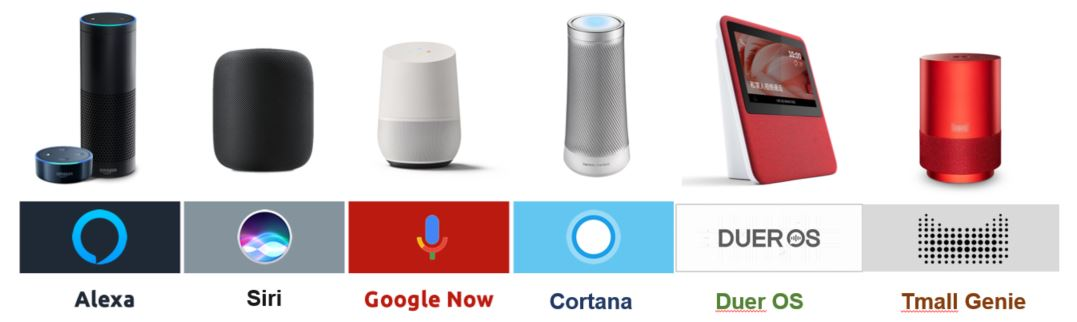
\includegraphics[width=1\linewidth]{Picture/Sprachassistenten}
	\caption[Sprachassisten auf dem MarkT]{Sprachassisten auf dem MarkT}
	\label{fig:sprachassistenten}
\end{figure}

Amazons Alexa verwendet alle Nutzereingabe, um den Sprachservice zu verbessern und personalisierte Werbung anzuzeigen. Eine Beschränkung der Datennutzung für verschiedene Bereiche ist möglich, wodurch sich allerdings auch die Funktionalität einschränkt \cite{alexaPrivacy}.

Google Assistant verwendet die gleichen Berechtigungen, welche für die mobile App des Anbieters gelten \cite{googleShare}. Eine abweichende Einstellung zur mobilen App ist dabei nicht möglich. Die Interaktion mit Google Assistant kann für die personalisierte Werbung genutzt werden, wie sonstige Suchanfragen \cite{googlePrivacy}.

Bei Siri müssen Dienste aktiviert sein, um darauf zurückgreifen zu können. Um die Aussprache und die Funktionalität zu verbessern, werden Daten wie Name, Kontakte, Musik, Suchaktivitäten und weitere Informationen verschlüsselt übertragen. Die Daten werden nicht mit der Apple ID genutzt, sondern mit zufällig erstellter Kennung. Dadurch wird Privatsphäre für Nutzer gewährleistet \cite{siriPrivacy}.

In den Datenschutzeinstellungen von Microsofts Cortana wird darüber informiert, dass bestimmte Daten \glqq [...] wie z. B. Ihre Suchen, Kalender, Kontakte und Orte. [...]\grqq{} gespeichert werden. Die Datennutzung von Cortana als Personal Assistant ist konfigurierbar. Sind die personalisierten Informationen deaktiviert, kann Cortana nur für Anwendungen wie der Suche und des Festlegung eines Timers genutzt werden. Cortana verwendet personenbezogene Daten nicht für personalisierte Werbung \cite{cortanaAssistent}. 

Baidu DuerOS sammelt ebenfalls Nutzerdaten, um die Sprachverarbeitung des Sprachassistenten zu verbessern. Qi Lu verweist auf die vielen Szenarien in denen Baidu Daten sammelt, womit Baidu den Sprung an die Weltspitze im Bereich Künstliche Intelligenz gelingen soll . Die persönlichen Daten eines Nutzers werden übermittelt. Dabei bietet Baidu keine konfigurierbare Privatsphäre an \cite{baiduAI}. 

Seit Februar gibt es den Sprachassistenten Mycroft Mark II, indem Offenheit und Privatsphäre vereint werden \cite{mycroftsmartspeaker}. Die Funktionalitäten sind hier begrenzt, da der Sprachassistent keine Daten speichert um den Benutzerkontext weiter zu trainieren und zu verstehen.
\section{Motivation}\label{sec:motivaiton}
A survey was conducted to check whether more privacy was desired for voice assistants. 110 participants took part in the survey. The participants included the following age groups:
\begin{itemize}
	\item 0 to 18 years 
	\item 19 to 25 years
	\item 26 to 35 years
	\item 36 and older	
\end{itemize}

\begin{figure}[h]
	\centering
	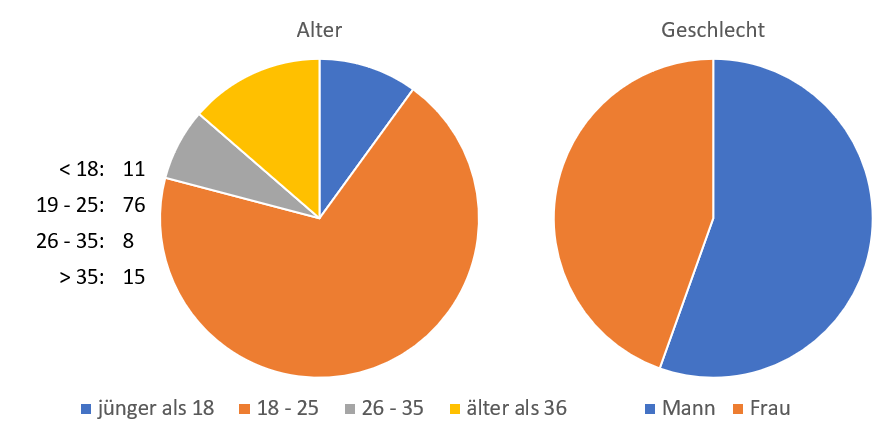
\includegraphics[width=0.9\linewidth]{Picture/umfrage_teilnehmer}
	\caption[Participant of the survey]{Participant of the survey}
	\label{fig:umfrage_teilnehmer}
\end{figure}

55.5\% of the participants were male and 45.5\% female, as shown in Figure \ref{fig:umfrage_teilnehmer}. The participants were asked the following questions:

\begin{enumerate}	
	\item How often do you use a voice assistant?
	\item Do you know what happens to your personal data?
	\item Would you pay money for better data security?
	\item How much money would you pay once for a better data security of an application?
	\item In which applications is privacy especially important to you?
\end{enumerate}

The result of the first question was that 44.5\% of participants use a voice assistant once a month or more frequently. In the US, a study of "highervisibility" was conducted, in which more than 70\% of participants use a voice assistant once a month or more \cite{highervisibility}.

A direct comparison of the survey with the study from the USA is shown in Figure \ref{fig: survey_base}. In the study, people in different age groups from different backgrounds were interviewed. The survey conducted under this article was mostly answered by young people.
\begin{figure}[h]
	\centering
	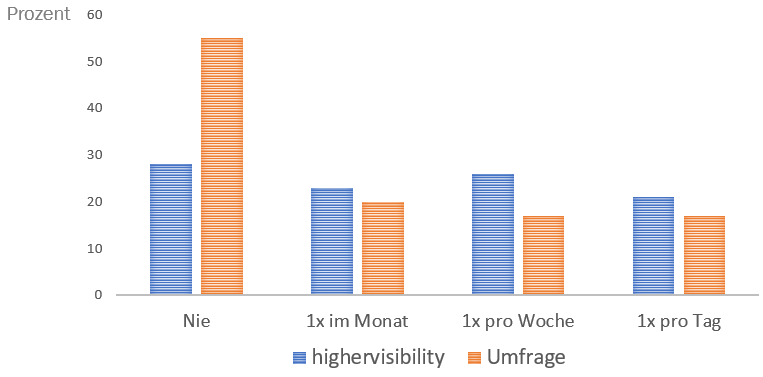
\includegraphics[width=0.9\linewidth]{Picture/umfrage_haeufigkeit}
	\caption[Frequency of use of voice assistants]{Frequency of use of voice assistants}
	\label{fig: survey_base}
\end{figure} 

As can be seen in figure \ref{fig:umfrage_datenschutz}, 90\% of the participants do not know what's happening to their data. The willingness to pay is visualized by age group in Figure \ref{fig:umfrage_geld_gruppen}. One in four would pay for better data security and 56\% of the participants are unsure whether they would spend money on it. The age rating after willingness to pay is lowest for the group under 18 years. The intersection of participants who ticked "Yes" or "Maybe" increases with age.

\begin{figure}[h]
	\centering
	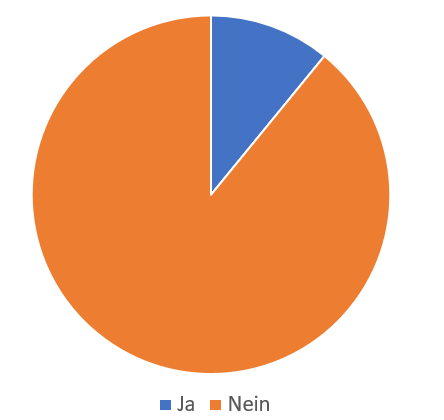
\includegraphics[width=0.5\linewidth]{Picture/umfrage_datenschutz}
	\caption[Relevance of data protection]{Relevance of data protection}
	\label{fig:umfrage_datenschutz}
\end{figure}

\begin{figure}[h]
	\centering
	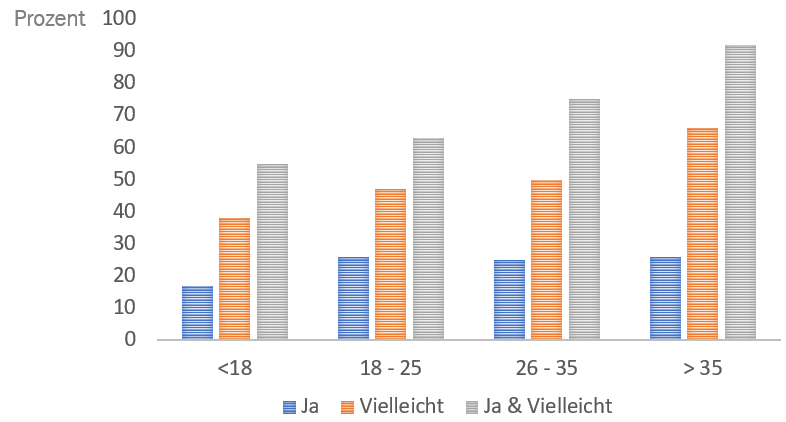
\includegraphics[width=0.9\linewidth]{Picture/umfrage_geld_gruppen}
	\caption[Willingness to pay of different age groups]{Willingness to pay of different age groups}
	\label{fig:umfrage_geld_gruppen}
\end{figure}

The amount that the participants would spend on applications varies a lot and can be seen in figure \ref{fig:umfrage_betrag}. About 15\% of participants are unwilling to pay, while a majority are ready to pay.

\begin{figure}[h]
	\centering
	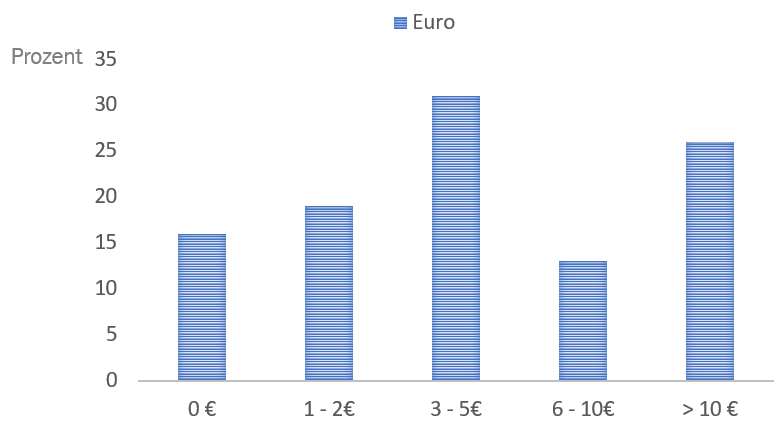
\includegraphics[width=0.9\linewidth]{Picture/umfrage_betrag}
	\caption[Willingness to pay by amount]{Willingness to pay by amount}
	\label{fig:umfrage_betrag}
\end{figure}

As shown in figure \ref{survey_application}, the privacy of applications like banking, home automation, handset control, social networking and chatting is particularly important to the participants.

\begin{figure}[h]
	\centering
	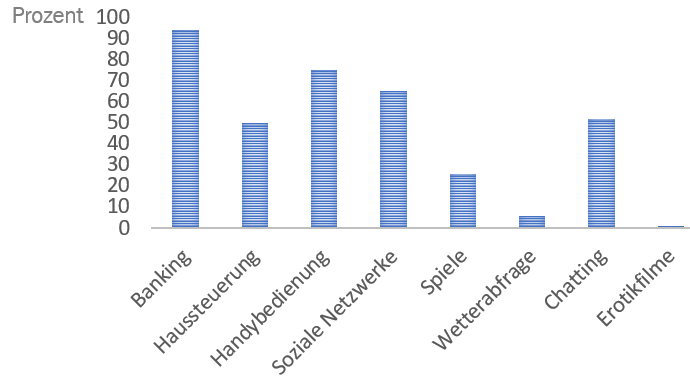
\includegraphics[width=0.9\linewidth]{Picture/umfrage_anwendung}
	\caption[Data protection relevant applications]{Data protection relevant applications}
	\label{survey_application}
\end{figure}

From the survey, the following conclusions can be drawn:
\begin{itemize}	
	\item Some people use voice assistants
	\item Users do not know what's happening to their data
	\item Users would pay for an application if it protects their data
	\item Data protection is important in the areas of banking, chatting, home automation, social media and mobile control.
\end{itemize}

\section{Konzept}\label{sec:konzept}
\section{Architektur}\label{sec:architecure}
Nun gilt es das in Kapitel \ref{sec:konzept} vorgestellte Konzept umzusetzen. Dazu wurde eine Architektur für einen Sprachassistenten entwickelt, welche in Abbildung \ref{fig:infrastruktur-overview} zu sehen ist. Diese Architektur bietet mehr Privatsphäre und ist unterteilt in drei Hauptmodule: Die Mobile App, das Repository und die Cloud. Dabei existiert das Modul \glqq Speech Processing\grqq{} in der Mobilen App und in der Cloud. In der Mobilen App werden einfache Sprachverarbeitungsprozesse wie beispielsweise das Aufnehmen bzw. die Wiedergabe eines Audiofiles implementiert. Ressourcenintensive Sprachverarbeitungsprozesse, wie beispielsweise die Umwandlung von Sprache zu Text, werden in die Cloud ausgelagert. Im Folgenden sind die drei Hauptmodule genauer beschrieben.
\begin{figure}[h!]
	\centering
	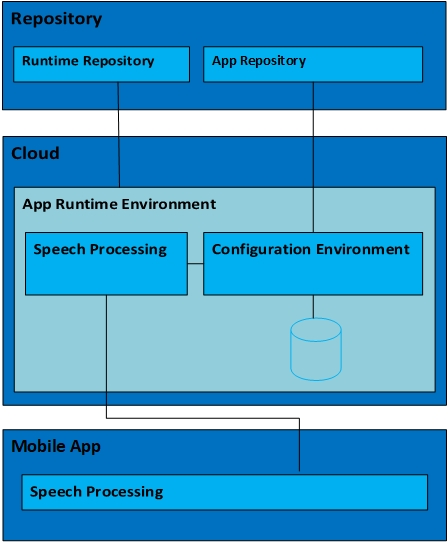
\includegraphics[width=0.8\linewidth]{Picture/Infrastruktur-Overview.jpg}
	\caption[Architekturübersicht]{Architekturübersicht}
	\label{fig:infrastruktur-overview}
\end{figure}

\subsection{Mobile App}
Die Mobile App ist die Schnittstelle zum Nutzer und wie Abbildung \ref{fig:infrastruktur-app} zeigt, hat diese drei Module:

\begin{description}
	\item \textit{Speech Recording}: Aufnehmen und streamen der Eingabe eines Nutzers an die Cloud.
	\item \textit{Speech Playback}: Abspielen eines Streams, der von der Cloud erzeugt wurde, an den Nutzer.
	\item \textit{Hotword Detection}: Die Mobile App soll nicht ununterbrochen die Eingabe des Nutzers an die Cloud streamen, denn dies könnte die Privatsphäre des Nutzers beeinträchtigen. Die App soll nur aufnehmen und streamen, wenn der Nutzer das will. Somit kommt die sogenannte \glqq Hotword Detection\grqq{} zum Einsatz. Diese belauscht den Nutzer durchgängig lokal auf dem Endgerät. Eine Hotword Detection benötigt kaum Ressourcen, da sie für die Erkennung eines einzigen Signalwortes optimiert wurde. Somit lässt sich ein Signalwort definieren, mit dem das Aufnehmen bzw. streamen an die Cloud gestartet wird. 
\end{description}

\begin{figure}[h!]
	\centering
	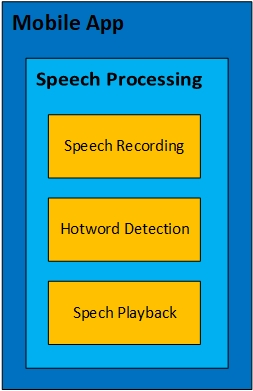
\includegraphics[width=0.3\linewidth]{Picture/Infrastruktur-App.jpg}
	\caption[Architektur - Mobile App]{Architektur - Mobile App}
	\label{fig:infrastruktur-app}
\end{figure}

\subsection{Repository}
Das Repository ist in Abbildung \ref{fig:infrastruktur-repository} dargestellt und unterteilt sich nochmals in zwei Module: Das Runtime Repository und das App Repository, welche im folgenden genauer beschrieben werden.

\begin{description}
	\item \textit{Runtime Repository}: Das Runtime Repository stellt eine Laufzeitumgebung für die Cloud bereit. Die Laufzeitumgebung beinhaltet das Betriebssystem und alle vom Sprachassistenten benötigten Pakete und wird in verschieden Formaten bereitgestellt. Ein Nutzer kann eine Laufzeitumgebung im Format seiner Wahl herunterladen und auf seiner privaten Cloud installieren. Dabei soll die Installation möglichst wenig Konfigurationsaufwand erfordern, denn auch Nutzer ohne IT-Background sollen sich diese Umgebungen installieren können. 
	\item \textit{App Repository}: Das App Repository stellt alle Apps bereit, die für den Sprachassistenten verfügbar sind. Will ein Nutzer ein App nutzen, so muss er diese in seiner Laufzeitumgebung installieren. Entwickler können Apps im App Repository für Nutzer bereitstellen. Jedoch müssen diese exakte Angaben über die Nutzung der Daten eines Nutzers tätigen. Des Weiteren wird vor einer Veröffentlichung einer App geprüft, ob die Angaben zum Datenschutz korrekt sind und ob diese erfassten Daten überhaupt für die Verbesserung der Nutzerfreundlichkeit notwendig sind. Somit lässt sich Datensparsamkeit für eine App erreichen.
\end{description}


\begin{figure}[h!]
	\centering
	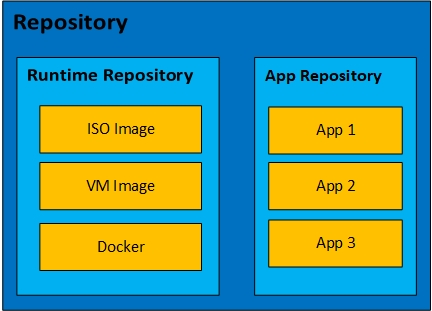
\includegraphics[width=0.6\linewidth]{Picture/Infrastruktur-Repository.jpg}
	\caption[Architektur - Mobile App]{Architektur - Repository}
	\label{fig:infrastruktur-repository}
\end{figure}

\subsection{Laufzeitumgebung}
Die Laufzeitumgebung ist das Herzstück des Sprachassistenten und ist in Abbildung \ref{fig:infrastruktur-cloud} aufgezeigt. Sie beinhaltet einen großen Umfang an Funktionen.

\begin{figure}[h!]
	\centering
	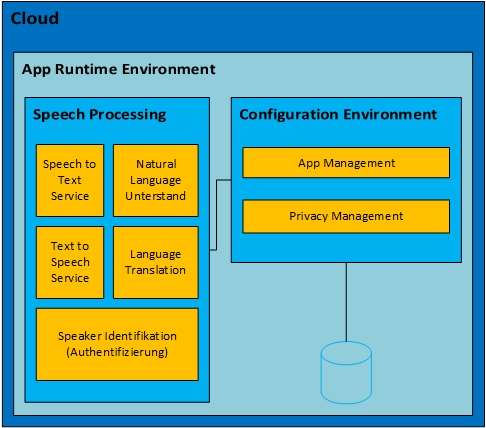
\includegraphics[width=0.9\linewidth]{Picture/Infrastruktur-Cloud.jpg}
	\caption[Architektur - Mobile App]{Architektur - Cloud}
	\label{fig:infrastruktur-cloud}
\end{figure}

\begin{description}
	\item \textit{Sprachverarbeitung}: Das Modul Speech Processing beinhaltet rechenintensive Funktionen der Sprachverarbeitung. Folgende Teilgebiete der Sprachverarbeitung werden für den Sprachassistenten benötigt:
	\begin{itemize}
		\item \ac{stt}: \ac{stt} ist die Umwandlung eines Sprachsignals zu Text.
		\item \ac{tts}: \ac{tts} ist die Umwandlung eines Text zu einem Sprachsignal.
		\item \ac{nlu}: \ac{nlu} ist das Verständnis der natürlichen Sprache. Dies ist nötig, um die Eingabe eines Nutzers zu verstehen. Es kann beispielsweise erkannt werden, ob ein Wort in einem Satz ein Nomen oder Verb ist. 
		\item Language Translation: Hierbei geht es um die Übersetzung eines Texts in eine andere Sprache. Damit kann ein Nutzer mit Nutzern, die eine andere Sprache sprechen kommunizieren. Eine App für den Sprachassistenten kann nicht in der Sprache des Nutzer zur Verfügung stehen, jedoch können die Inhalte der App zur Laufzeit in die Sprache des Nutzers übersetzt werden. Dies minimiert den Entwicklungsaufwand von Apps und erlaubt gleichzeitig das Erreichen einer große Zielgruppe an Nutzern, welche unterschiedlichste Sprachen sprechen. 
		\item Speaker Identifikation: Die Sprecheridentifikation kann als Authentifizierungsmethode des Sprachassistenten dienen. Durch die Sprachinformation in einem Sprachsignal eines Nutzers kann dieser identifiziert werden. Somit kann geprüft werden, ob ein Nutzer die Berechtigung hat, diesen Sprachassistenten zu nutzen.
	\end{itemize}
	\item \textit{Konfigurationsumgebung}: Über die Konfigurationsumgebung lassen sich die Apps- und Privatsphäre-Einstellungen für den Sprachassistenten vornehmen.
	\begin{itemize}
		\item App Management: Dieses Modul verwaltet die vom Nutzer installierten Apps. Dabei können neue Apps aus dem App Repository installiert oder vorhandene Apps deinstalliert werden.
		\item Privacy Management: Dieses Modul verwaltet den Kontext des Nutzers und erlaubt diesem, den Zugriff von Apps auf diesen Kontext festzulegen. Dabei kann bestimmt werden, welche Informationen des Nutzer von einer App zugänglich sind. Des Weiteren lassen sich auch fiktive Kontexte erstellen, sodass der Nutzer ohne Preisgabe seines tatsächlichen Kontexts eine App nutzen kann. Durch dieses Modul kann User-Controlled-Privacy erreicht werden. 
	\end{itemize}	
\end{description}






\section{Implementation}\label{sec:umsetzung}
This chapter identifies technologies that can be used to implement the architecture presented in the last chapter.

\subsection{Mobile App}
The mobile app will be implemented for various mobile platforms such as Android, iOS, Windows Phone and as a web application. Furthermore, the mobile app can also be integrated into a loudspeaker.
\begin{itemize}
	\item \textsl{Speech Recording:} Recording a user's input does not require additional technology in most cases. Almost all mobile devices already have a microphone and the device \acs{sdk} provides an interface to access the microphone.
	\item \textsl{Speech Playback:} Also for playing a stream, the built-in speaker can be used via the devices \acs{sdk}.
	\item \textsl{Hotword Detection:} The following are technologies that can be used to detect a signal word on the mobile device:
	\begin{itemize}
		\item Snowboy Hotword Detection from Kitt.ai: Snowboy Hotword Detection is an Apache licensed software project for detecting a signal word. The signal word can be determined freely and the software project is optimized for embedded systems. According to the manufacturer Kitt.ai, the hotword detection under the smallest Raspberry Pi (single-core 700MHz ARMv6) is only consuming 10\% of the CPU \cite{SnowboyHotwordDetection}.
		\item Sensory's TrulyHandsfreeTM: Sensory's TrulyHandsfreeTM is a speech recognition optimized for recognizing single words or a signal word. It also shows very good results in environments with lots of background noise. The vocabulary to be recognized can be created by Sensory's Grammar Tool. Sensory's TrulyHandsfreeTM is available for Android, iOS, QNX, Windows and microcontrollers \cite{TrulyHandsfreeTM}.
		\item Pocketsphinx from \acs{cmu} Sphinx: Sphinx is a \ac{cmu} research project dealing with speech recognition. Sphinx is based on the Open Source license and can therefore be used freely as long as it is acknowledged that it is a software of \ac{cmu}. Pocketsphinx, as well as Sensory's TrulyHandsfreeTM, has been optimized to recognize single words or a signal word \cite{Pocketsphinx}.
	\end{itemize}
\end{itemize}

\subsection{Repository}
The repository can be implemented by a web server. This web server provides on the one hand different runtime environments and on the other hand apps for the voice assistant for download. The runtime environments can be offered in the following formats:
\begin{itemize}
	\item \textsl{VMWare Image:} The VMWare image already contains a preinstalled operating system as well as all necessary packages for the voice assistant. A user must import this image into their VMWare environment (VMWare vSphere, Workstation, Player) and make only small network configurations. This environment is easy to use and requires the least amount of configuration. In addition, the user has the option of transferring the virtual machine to another server or taking snapshots. Snapshots are images of a virtual machine that reflect a particular state. This can easily jump back to the last functional snapshot in case of a misconfiguration \cite{VMWare}.
	\item \textsl{Docker Image:} The Docker Image is a configuration file for a container environment. This configuration file contains all packages and configurations for the voice assistant to be installed. If this configuration file is started in a container environment, the packages are automatically installed and the voice assistant is configured. The user only has to make network settings to use the voice assistant \cite{Docker}.
	\item \textsl{\acs{iso}-Image:} The \acs{iso}-Image provides the user with the most flexibility and configuration. The user can decide whether to install the runtime environment physically or virtualized. Furthermore, this is not tied to virtualization software like VMWare. It can be virtualized on a private or public cloud. A public cloud relieves the user of tasks such as visualization, backups, reliability and load balancing. Possible providers are \ac{aws} with Amazon EC2 \cite{AWSAmazonEC2}, Microsoft Azure \ cite {MicrosoftAzure}, and IBM Bluemix \cite{IBMBluemix}. The \acs{iso}-Image also contains all the necessary packages for the voice assistant. The user is guided through a wizard during the installation of the \acs{iso}-Image, where all configurations are made.
\end{itemize}

\subsection{Runtime Environment}
\subsubsection{Speech Processing}
In the runtime environment, speech processing processes are performed. There are two ways to perform these processes, either locally on the runtime environment or through the use of voice-based cloud services. The advantages and disadvantages as well as possible technologies of these possibilities are explained below.
\begin{itemize}
	\item \textsl{Cloud-based Speech Processing:} The use of voice-based cloud services for speech processing provides the best possible performance. The speech processing is based on a \ac{ai}, which improves with input data. Because cloud services are used by many applications, \ac{ai} provides a large amount of input data. The disadvantage of this is that a user's \ac{ai} input data describing its context is used to improve the \ac{ai}. Thus, the privacy is not optimally protected. Furthermore, the use of cloud services incurs costs. The following providers offer voice-based cloud services:
	\begin{itemize}
		\item \ac{aws}: Amazon offers many voice-based cloud services. Amazon Comprehend is a service for \ac{nlu}, gaining insight into the context and relationships of a text \cite{AmazonComprehed}. With Amazon Translate, texts, web pages, and applications can be translated naturally and accurately \cite{AmazonTranslate}. Amazon Transcript can convert speech to text and Amazon Polly text to speech \cite{AmazonTranscript} \cite {AmazonPolly}. Amazon Lex can create conversation interfaces for applications. A chat bot serves as a  interface and can generate the corresponding answer to a specific input. Amazon Lex uses the same deep learning algorithms as voice assistant Alexa from Amazon \cite{AmazonLex}.
		\item Microsoft Azure: Microsoft Azure offers cognitive services, including text to speech, speech to text, text translation, and \ac{nlu} services. It also offers a speaker recognition and spelling correction service \cite{MicrosoftAzureCognitiveServices}. Speech recognition is an important part of the concept of the voice assistant presented in this article. Through this service, a user can be authenticated.
		\item IBM Watson: IBM Watson also offers voice-based cloud services for speech to text and text to speech conversion. Furthermore, a service for \ac{nlu} and \ac{nlc} is offered. By \ac{nlc} the intention of an input can be determined. With Watson Assistant a Chat bot can be realized \cite{IBMWatsonSpeechServices}.
	\end{itemize}
	\item \textsl{Local Speech Processing:} The use of local speech processing in the runtime environment provides better control of the user's privacy. This requires significantly more resources on the runtime environment, and performance is usually worse than using voice-based cloud services. There are some vendors that offer frameworks for local speech processing. Including open-source projects, resulting in no costs for the use.
	\begin{itemize}
		\item Nuance:Nuance has been working on speech processing solutions for over 25 years, focusing on integrating these solutions into mobile devices such as smartphones or cars. Among other things, solutions for speech to text and text to speech conversions and to create a chat bot are offered \cite{Nuance}. 
		\item Mozilla: Mozilla is launching the Common Voice project, an initiative to help teach machines the way real people speak. This initiative is still under development. Currently, records are being collected to improve the \ac{ai}. The initiative is considered as an open source project and each person can add records for improvement of the \ac{ai}. For this purpose, Mozilla has created a website and mobile app with the contributor to review records or input data \cite{MozillaCommonVoice}. The potential of this initiative will only become apparent after the end of development.
		\item Kaldi: Kaldi is a speech recognition toolkit that is freely available under the Apache license. Kaldi aims to deliver software that is flexible and extensible \cite{Kaldi}. The project is managed on GitHub, so developers can help improve the toolkit.
		\item CMUSphinx: CMUSphinx offers with Pocketsphinx a speaker-independent continuous speech recognition. Pocketsphinx is an open source project and is managed on GitHub. Pocketsphinx can be used in mobile devices, offering a version for smartwatches that does not require an internet connection. Finished models for the \ac{ai} are offered, but even own models can be trained \cite{Pocketsphinx}.
	\end{itemize}
\end{itemize}

\subsubsection{Configuration Environment}
The configuration environment can be realized by a web application. The user can configure his voice assistant via any device with a browser. Furthermore, these configurations can also be done with the mobile app. Figure \ref{fig: prototype} shows a prototype of what this mobile app might look like. In doing so, a user can view his context and determine which contextual information of apps may be used. The user can manipulate his context if certain information is needed by an app; he does not want to divulge these for reasons of privacy. Thus, the user has full control over his data.

\begin{figure}[!ht]
	\centering
	\begin{subfigure}{0.32\linewidth}
		\centering
		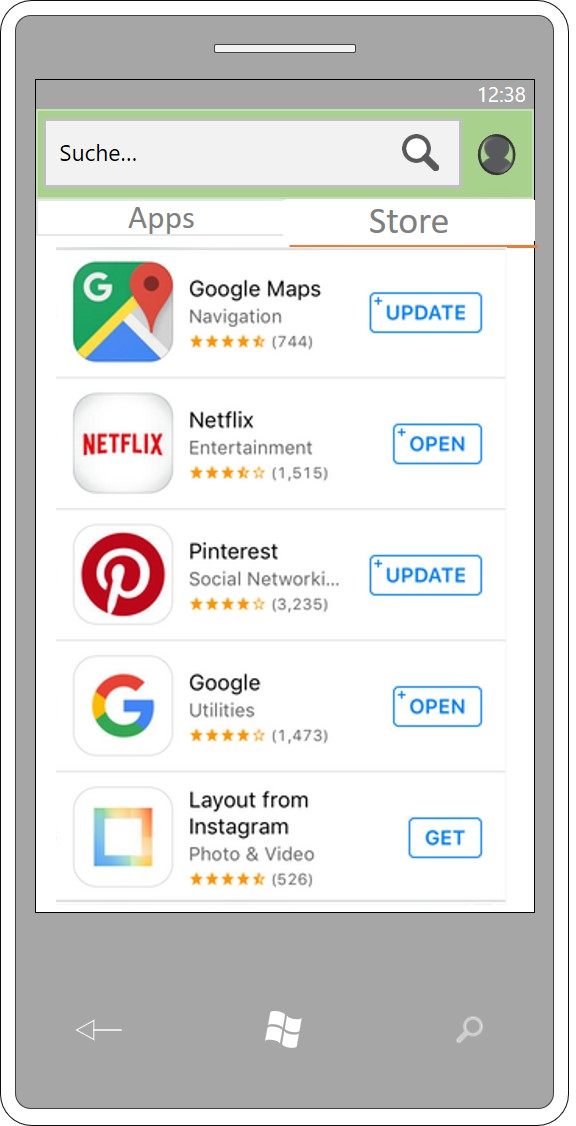
\includegraphics[width=1\linewidth]{Picture/App-Store}
		\caption{Mobile App - Store}
		\label{fig:prototyp1}
	\end{subfigure}%
	\begin{subfigure}{0.32\linewidth}
		\centering
		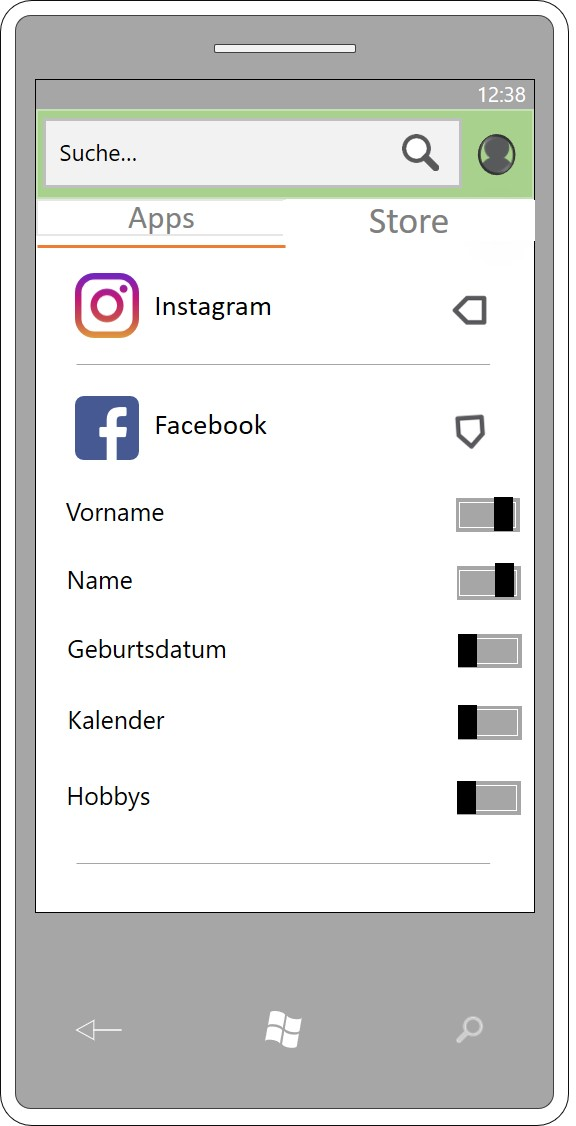
\includegraphics[width=1\linewidth]{Picture/App-Settings}
		\caption{Mobile App - Settings}
		\label{fig:prototyp2}
	\end{subfigure}
	\begin{subfigure}{0.32\linewidth}
		\centering
		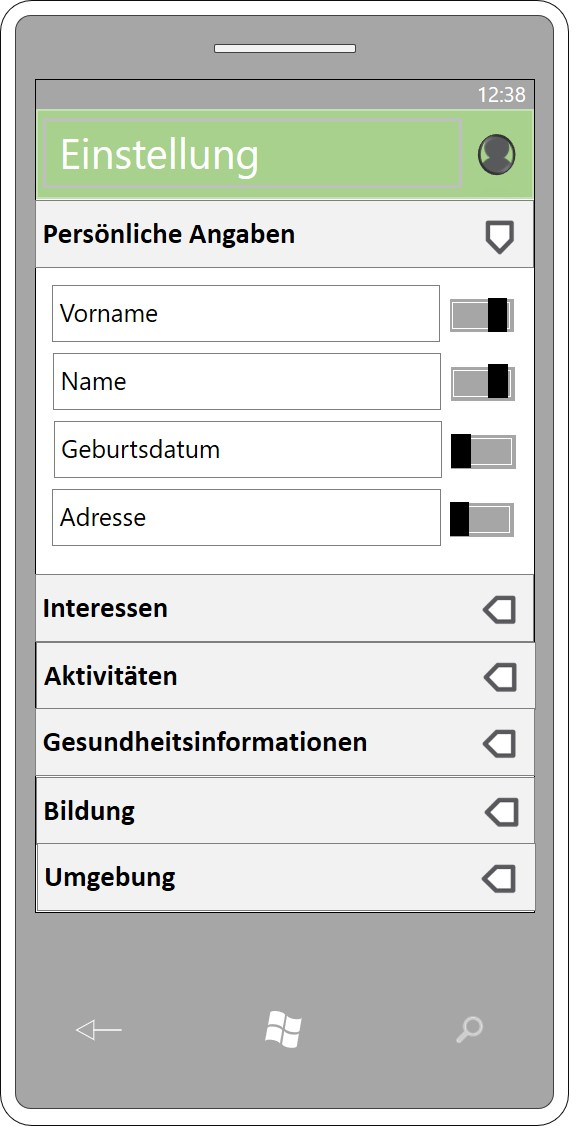
\includegraphics[width=1\linewidth]{Picture/App-Kontext}
		\caption{Mobile App - User Context}
		\label{fig:prototyp3}
	\end{subfigure}%
	\caption{Prototyp of the mobile App}
	\label{fig:prototyp}
\end{figure}












\section{Future Work}
This article highlights the problem of current voice assistants. With the presented concept the user can be guaranteed a better privacy. The last chapter presented some technologies for implementing this concept. It turned out that there is a wide range of technologies in the field of speech processing. As a next step, these technologies would need to be evaluated to make a technology selection. This selection can be used to determine what resources the private cloud needs to use these technologies. Furthermore, a cost model can be created based on the required resources and technologies. This can be used to conduct a new survey or interviews with potential target groups. The survey aims to show if the target groups are willing to pay additional costs for better privacy. Then you can start with a prototypical development of the voice assistant. In addition, a concept has to be developed with which apps can be checked for unwanted data transfer to third parties.
\section{Zusammenfassung}

Die Umfrage hat eine gute Übersicht über die aktuelle Verwendung von Sprachassistenten gegeben. Zwar ist die Teilnehmerzahl nicht sonderlich groß, auf die Region beschränkt und im Alter nicht ausreichend verteilt, aber ein Stimmungsbild kann dennoch erkannt werden. Die Personen aus der Region Freiburg nutzen mehrheitlich keinen Sprachassistenten. Der Datenschutz ist den Teilnehmern wichtig, wobei mehr als 25\% Geld dafür bezahlen würde. 

 Grundsätzlich ist das Konzept unserer Ansicht nach gelungen, da der Benutzer im Mittelpunkt agiert und je nach Anwendung entscheiden kann, ob Privacy oder Funktionalität überwiegt. Große Anbieter sollten ein ebenfalls zahlungspflichtiges Modell etablieren, in welchem die Nutzer im die Entscheidungen über Privacy und Funktionalität treffen können. 

Die Architektur ist so gestaltet, dass ein solcher Sprachassistent einfach im Betrieb genommen werden kann. Allerdings lässt sich das vorgestellte Konzept nach heutigem Stand schwer umsetzen, da der Nutzer viele Ressourcen für die Verarbeitung benötigen. 

Es sind bereits viele Open-Source-Unterstützungen vorhanden, sodass die Umsetzung erleichtert wird. 
\section{Danksagung}
Diese Artikel wurde im Rahmen des Moduls \glqq Mobilität und Innovation\grqq{} an der Fachhochschule Furtwangen und unter Betreuung von Prof. Dr. Achim P. Karduck erstellt, dem wir für die gute Betreuung und die vielen Denkanstöße danken.
% *** END OF SECTIONS ***---------------------------------------------


% Can use something like this to put references on a page
% by themselves when using endfloat and the captionsoff option.
\ifCLASSOPTIONcaptionsoff
  \newpage
\fi

\begin{thebibliography}{1}
\bibitem{Campaign}
Christi Olson: "Just say it: The furture of search is voice and personal digital assistant", Campaign 25.04.2016 \url{https://www.campaignlive.co.uk/article/just-say-it-future-search-voice-personal-digital-assistants/1392459},
Zuletzt besucht: 13.07.2018

\bibitem{prNewswire}
OC\&C Strategy Consultants: "Voice Shopping Set to Jump to \$40 Billion By 2022, Rising From \$2 Billion Today", PR Newswire, 28.02.2018, \url{https://www.prnewswire.com/news-releases/voice-shopping-set-to-jump-to-40-billion-by-2022-rising-from-2-billion-today-300605596.html}, 
Zuletzt besucht: 13.07.2018

\bibitem{highervisibility}
Adam Heitzman: "How popular is voice search?", 07.02.2017, higervisibility.com, \url{https://www.highervisibility.com/blog/how-popular-is-voice-search/},
Zuletzt besucht: 13.07.2018

\bibitem{homeAssistants}
”Choosing The Best Voice Assistant For Your Home”, Geeks of Technology,
16.01.2018, \url{https://geeksfl.com/blog/best-voice-assistant/}, Last visit:
20.07.2018 .

\bibitem{kairannenberg}
Rannenberg, Kai. "Mehrseitige Sicherheit—Schutz für Unternehmen und ihre Partner im Internet." Wirtschaftsinformatik 42.6 (2000): 489-497.

\bibitem{cortanaAssistent}
Mircosoft Inc: "Cortana, Ihre persönliche digitale Assistentin", \url{https://privacy.microsoft.com/de-de/windows-10-cortana-and-privacy},
Zuletzt besucht: 05.06.2018

\bibitem{siriAssistent}
Apple Inc.: "Hey Siri, weck mich morgen früh um 7:00 Uhr.",
\url{https://www.apple.com/de/ios/siri/},
Zuletzt besucht: 05.06.2018

\bibitem{alexaAssitent}
Amazon Inc.: "Alexa Assistant"
\url{https://www.amazon.de/b?ie=UTF8&node=12775495031},
Zuletzt besucht: 06.06.2018

\bibitem{alexaPrivacy}
Amazon Inc.: "Alexa Internet Privacy Notice", 23.05.2018,
\url{https://www.alexa.com/help/privacy},
Zuletzt besucht: 06.06.2018

\bibitem{googleAssistant}
Google LLC: "Google Assistant - Just say" ,
\url{https://assistant.google.com/#?modal_active=none},
Zuletzt besucht: 06.06.2018

\bibitem{googlePrivacy}
Google LLC: "Datenschutzerklärung \& Nutzungsbedingungen", 25.05.2018, \url{https://policies.google.com/privacy#whycollect},
Zuletzt besucht: 06.06.2018

\bibitem{baiduAssistant}
Baidu Inc.: "What makes our Artificial Intelligence technology unique"  \url{https://dueros.baidu.com/en/index.html},
Zuletzt besucht: 06.06.2018

\bibitem{baiduPrivacy}
Baidu Inc.: "Baidu Statement of Privacy Protection", \url{http://ir.baidu.com/phoenix.zhtml?c=188488\&p=privacy},
Zuletzt besucht: 06.06.2018


\bibitem{baiduAI}
Jessi hemple: "How Baidu will win china's AI race - and, maybe, the world's", 08.09.2017, \url{https://www.wired.com/story/how-baidu-will-win-chinas-ai-raceand-maybe-the-worlds/},
Zuletzt besucht: 06.06.2018

\bibitem{googleShare}
Google LLC: "Choose what to share with your Google Assistant", \url{https://support.google.com/assistant/answer/7126196?hl=en},
Zuletzt besucht: 06.06.2018

\bibitem{siriPrivacy}
Apple Inc.: "Umgang mit Datenschutz", \url{https://www.apple.com/de/privacy/approach-to-privacy/},
Zuletzt besucht: 06.06.2018

\bibitem{mycroftsmartspeaker}
Jack Wallen: "Mycroft Mark II offers something its digital assistant competitors can't: Privacy and openness", 14.02.2018, \url{https://www.techrepublic.com/article/mycroft-mark-ii-offers-consumers-what-other-digital-assistants-cant-privacy/},
Zuletzt besucht: 06.06.2018	
	
\bibitem{SnowboyHotwordDetection}
Kitt.ai: "Snowboy Hotword Detection",
\url{https://snowboy.kitt.ai/},
Zuletzt besucht: 10.07.2018

\bibitem{TrulyHandsfreeTM}
Sensory: "TrulyHandsfreeTM",
\url{http://www.sensory.com/products/embedded-software-and-sdks/},
Zuletzt besucht: 10.07.2018

\bibitem{VMWare}
"VMWare",
\url{https://www.vmware.com/},
Zuletzt besucht: 11.07.2018

\bibitem{Docker}
"Docker",
\url{https://www.docker.com/},
Zuletzt besucht: 11.07.2018

\bibitem{IBMBluemix}
IBM Bluemix: "Virtual Server",
\url{https://www.ibm.com/cloud/virtual-servers},
Zuletzt besucht: 11.07.2018

\bibitem{AWSAmazonEC2}
Amazon: "Amazon EC2",
\url{https://aws.amazon.com/de/ec2},
Zuletzt besucht: 11.07.2018

\bibitem{MicrosoftAzure}
Microsoft Azure: "Virtual Server",
\url{https://azure.microsoft.com/en-us/services/virtual-machines/},
Zuletzt besucht: 11.07.2018

\bibitem{AmazonComprehed}
Amazon: "Amazon Comprehed",
\url{https://aws.amazon.com/de/comprehend/},
Zuletzt besucht: 11.07.2018

\bibitem{AmazonTranslate}
Amazon: "Amazon Translate",
\url{https://aws.amazon.com/de/translate/},
Zuletzt besucht: 11.07.2018

\bibitem{AmazonTranscript}
Amazon: "Amazon Transcript",
\url{https://aws.amazon.com/de/transcribe/},
Zuletzt besucht: 11.07.2018

\bibitem{AmazonPolly}
Amazon: "Amazon Polly",
\url{https://aws.amazon.com/de/polly/},
Zuletzt besucht: 11.07.2018

\bibitem{AmazonLex}
Amazon: "Amazon Lex",
\url{https://aws.amazon.com/de/lex/},
Zuletzt besucht: 11.07.2018

\bibitem{MicrosoftAzureCognitiveServices}
Microsoft Azure: "Cognitive Services",
\url{https://azure.microsoft.com/en-us/services/cognitive-services/directory/speech/},
Zuletzt besucht: 11.07.2018

\bibitem{IBMWatsonSpeechServices}
IBM Watson: "Speech Services",
\url{https://www.ibm.com/watson/services/},
Zuletzt besucht: 11.07.2018

\bibitem{Nuance}
"Nuance",
\url{https://www.nuance.com},
Zuletzt besucht: 12.07.2018

\bibitem{MozillaCommonVoice}
"Mozilla Common Voice",
\url{https://voice.mozilla.org/de},
Zuletzt besucht: 12.07.2018

\bibitem{Kaldi}
"Kaldi",
\url{http://kaldi-asr.org/},
Zuletzt besucht: 12.07.2018

\bibitem{Pocketsphinx}
CMUSphinx: "Pocketsphinx"
\url{https://cmusphinx.github.io},
Zuletzt besucht: 12.07.2018
\end{thebibliography}

\end{document}


